\subsection{Storing, Converting, and Carrying Power} 

%\DTMnewdatestyle{dateupdated}{〈definition 〉
Answers to M\Alph{subsection} problems are on page \pageref{power_conversion_prob_answers}.  \textbf{\textcolor{red}{Updated \DTMnow.}}

%--------------------------------------------------------------------------------------------------------------
\begin{Exercise}
A 200 nF capacitor is charged by a 5~V supply through a $2\kohm$ resistor, starting at zero volts.  (a)~Graph both the current $I_C$ through the capacitor and the voltage $V_C$ across the capacitor as functions of time.  (b)~At what time does the capacitor voltage reach 90\% of the supply voltage?  (c)~What is the current through the resistor at the time you calculated in part (b)?
\end{Exercise}
\begin{Answer}
(b) $921~\mu$sec (c) $250~\mu$A
\end{Answer}


%--------------------------------------------------------------------------------------------------------------
\begin{Exercise}
In the circuit shown to the right, the capacitor is initially uncharged and both switches are open. 
 
\figuretoright{0.28}[scale=0.9]{M_problems/power_conversion/charge_and_short_capacitor.pdf} {
\begin{itemize}[nosep]
	\item At time $t=0$  switch S1 is moved up, connecting its common terminal to $+10$~V. 
	\item At time $t=15$ seconds, the voltmeter reads 7 volts.  At that time, switch S2 is closed. 
	\item At time $t=20$ seconds, S2 is opened and S1 is moved down, connecting its common terminal to ground.
	\end{itemize}
	\medskip
	(a) Draw a qualitative graph (no calculations required) showing both the capacitor's voltage $V_C(t)$ and its current $I_C(t)$.%
	Let current flowing down through the resistor be defined as positive.
	\medskip
	
	(b) From the data given, what is the value of the resistance $R$ in the circuit?
	}
Note: the separation between the positive and negative plates of a capacitor prevents electrons from ``jumping'' across the gap between the two sides.  However, the current \textit{in} one side is always equal to the current \text{out} of the other, so we routinely talk about the current ``through'' the capacitor---even though individual electrons aren't actually go \textit{through}.
\end{Exercise}
\begin{Answer}
(b) $26.5\kohm$
\end{Answer}


%--------------------------------------------------------------------------------------------------------------
\begin{Exercise}
The circuit to the right is a square wave generator like the one you built in Lab~\ref{lab_capacitors}.

\figuretoright{0.50}{M_problems/power_conversion/comparator_square_generator.pdf} {
	\begin{enumerate}[label=(\alph*),wide]
	\item Calculate the two possible values of the input terminal $V_+$, (the upper and lower threshold voltages) depending on the value of $V_\text{out}$.  You can assume $R_4 \approx 0$. 
	\item Draw graphs of voltage vs. time for $V_\text{out}, V_+$,  $V_-$, showing how they are synchronized.  
	\item Calculate the time $\Delta t_\text{fall}$ for $V_-$ to fall from the higher threshold voltage to the lower threshold voltage.  
	\item Calculate the time $\Delta t_\text{rise}$ for $V_-$ to rise from the lower threshold voltage to the higher threshold voltage.  
	\item Find the output frequency of the oscillator.  
	\end{enumerate}
}

\medskip
\textit{Note that on an exam, you might be given this drawing and asked to find the frequency, without being asked all the helpful leading questions (a) through (d).}
\end{Exercise}
\begin{Answer}
(a) 1.56 V, 2.66 V (c) $\Delta t_\text{fall} = 80~\mu$s  (d) $\Delta t_\text{rise} = 58~\mu$s (e) 7.25~kHz
\end{Answer}

%--------------------------------------------------------------------------------------------------------------
\begin{Exercise}
The circuit to the right shows a voltage source connected to a load via a 3:1 transformer. 

\figuretoright{0.38}{M_problems/power_conversion/transformer_narrow.pdf} {
	\begin{enumerate}[label=(\alph*),wide]
	\item What is the apparent resistance of the load ``seen'' by the source?
	\item What is the voltage across the transformer's primary coil?
	\item What is the average power delivered to the load resistor, as shown?
	\item If you could replace the transformer, what turns ratio would you choose to deliver the maximum power to the load resistor?
	\item What is the maximum power you could deliver to the load? 
	\end{enumerate}
}
\end{Exercise}
\begin{Answer}
(a) $144\ohm$ (b) 4.64 volts RMS (c) 150 mW (d) 6.12:1 (e) 240 mW 
\end{Answer}


%--------------------------------------------------------------------------------------------------------------
\begin{Exercise}
Do a little Googling for the 1N4001 diode you've been using in the lab and find (a)~its reverse breakdown voltage $V_R$ and (b)~the maximum steady current you can pass through it in the forward direction, above which it presumably starts to smoke.  Although you can surely get this information by asking Google or any chat bot ``what is the reverse breakdown voltage of a 1N4001 diode,'' I'd like you to instead hunt down the datasheet for the 1N4001 online (cite your source!) and get the info directly from there.   (I know I've already posted a datasheet for the 1N4001 on Box, but see if you can find a datasheet on your own.)
\end{Exercise}


%--------------------------------------------------------------------------------------------------------------
\begin{Exercise}
\label{prob_first_diode_resistor_with_steps}
Our goal in this problem is to analyze the circuit below, finding the voltage and current of each component.  We can't tell ahead of time if there is current through the diode or not, so we'll have to try both possibilities.  

\figuretoright{0.30}{M_problems/power_conversion/diode_circuit1.pdf} {
Assume for parts~(a) through~(d) that there is a forward current in the diode.  
\begin{enumerate}[label=(\alph*),nosep]
\item Assuming there is a forward current in the diode, what is the voltage $V_D$ across the diode?  
\item What are $V_{R1}$ and $V_{R2}$?  
\item What are $I_{R1}$ and $I_{R2}$?
\item What is it about your last three answers that is inconsistent, thus demonstrating that our assumption in part~(a) must be bogus?  
\end{enumerate}
}

Now assume instead that there is NO current in the diode.  
\begin{enumerate}[label=(\alph*),nosep,start=5]
\item Assuming NO current in the diode, does the diode behave like an open or like a short?  
\item Find $V_{R1}$, $V_{R2}$, and the current in the circuit.  
\item Are the voltages you found in part~(f) consistent with your assumption in part~(e)?
\end{enumerate}
\end{Exercise}
\begin{Answer}
(a) 2.2 V \\
(b) 2.8 V and 2.2 V \\
(c) 2.8 mA and 5.5 mA \\
(d) We can't have $I_{R2}>I_{R1}$, because the only way for that to be true would be the current through the diode to be \textit{negative}, that is, flowing in the reverse direction. That would directly contradict the assumption that the diode has a forward current. \\
(e)~open \\
(f)~$V_{R1}=3.57$~V; $V_{R2}=1.43$~V; $I_D=0.$
\end{Answer}


%--------------------------------------------------------------------------------------------------------------
\begin{Exercise}
\label{prob_diode_1_of_2}
For the circuit below on the left, find the voltages and currents for all resistors and for the diode.  (This problem is a lot like \ref{prob_first_diode_resistor_with_steps}, but here you are not being led through it step by step.) 

\hfill
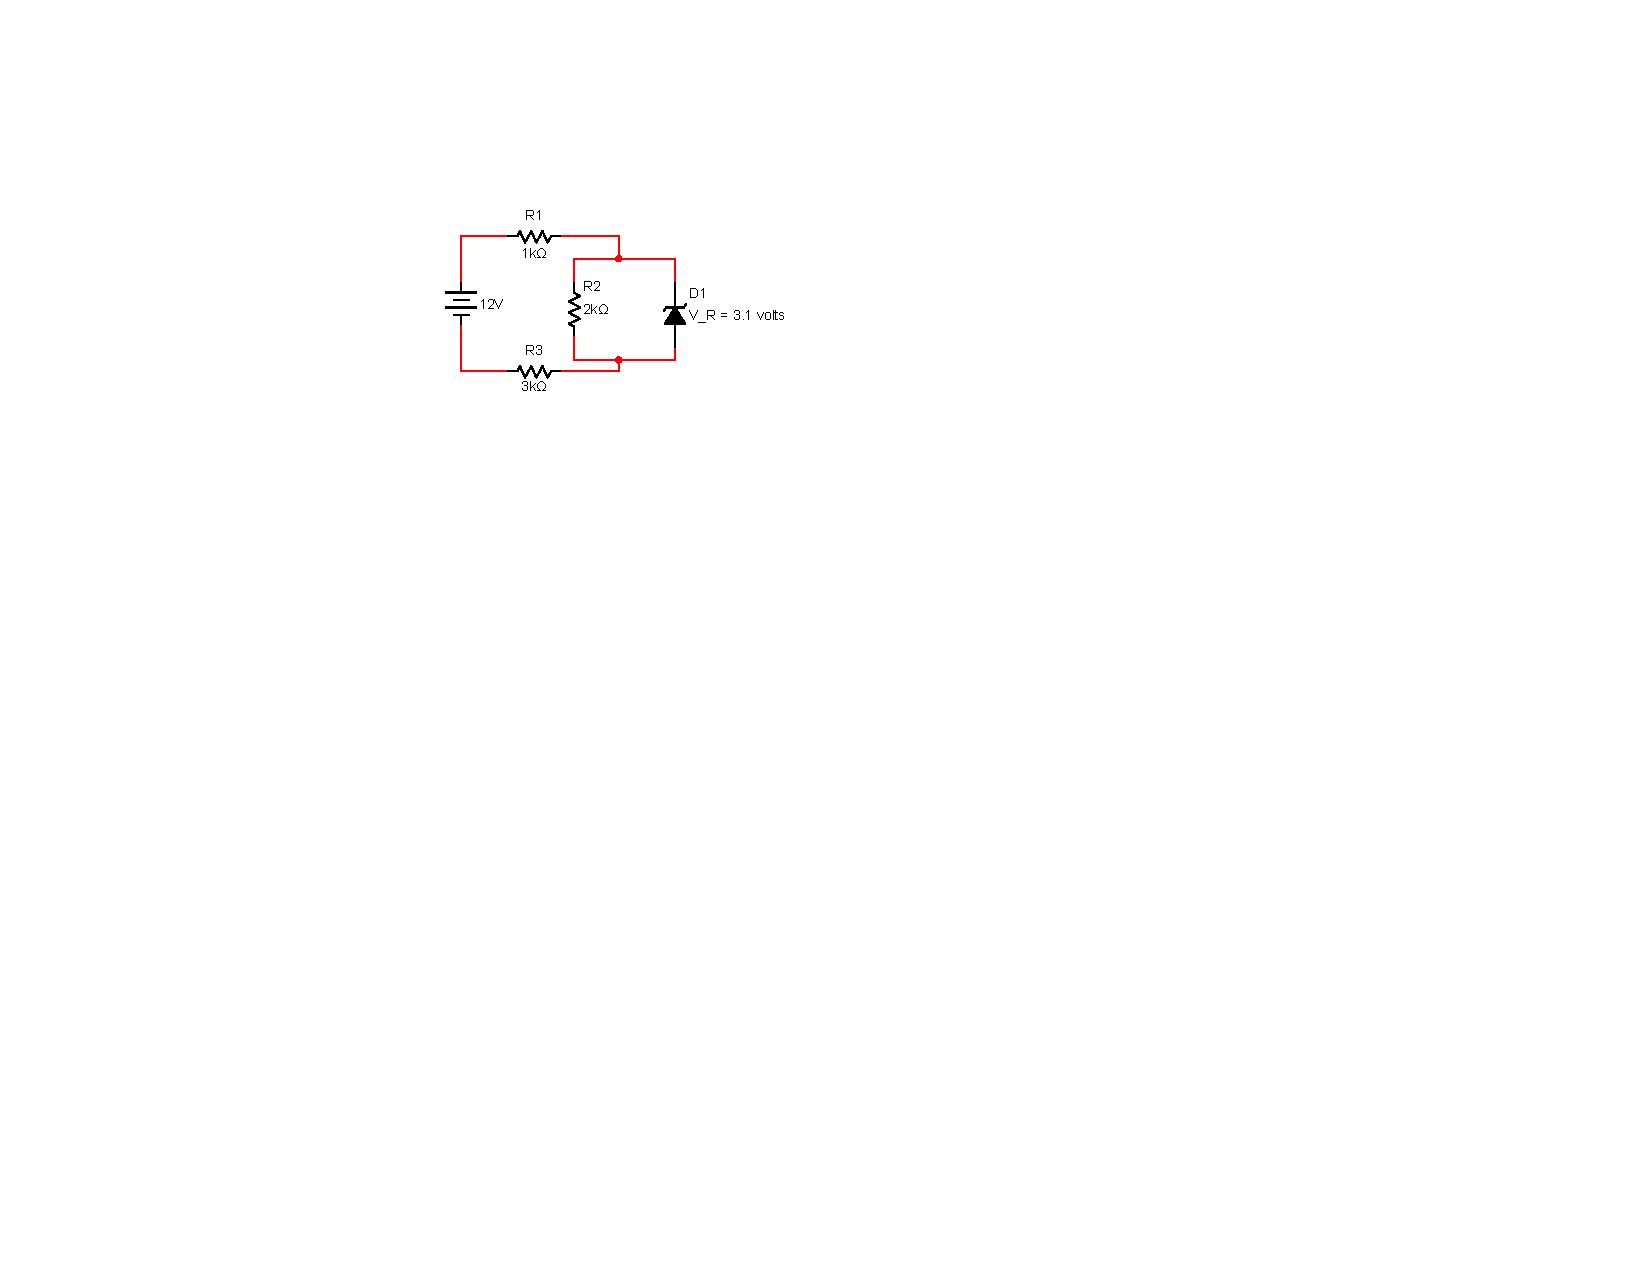
\includegraphics{M_problems/power_conversion/diode_circuit2.pdf}
\hfill
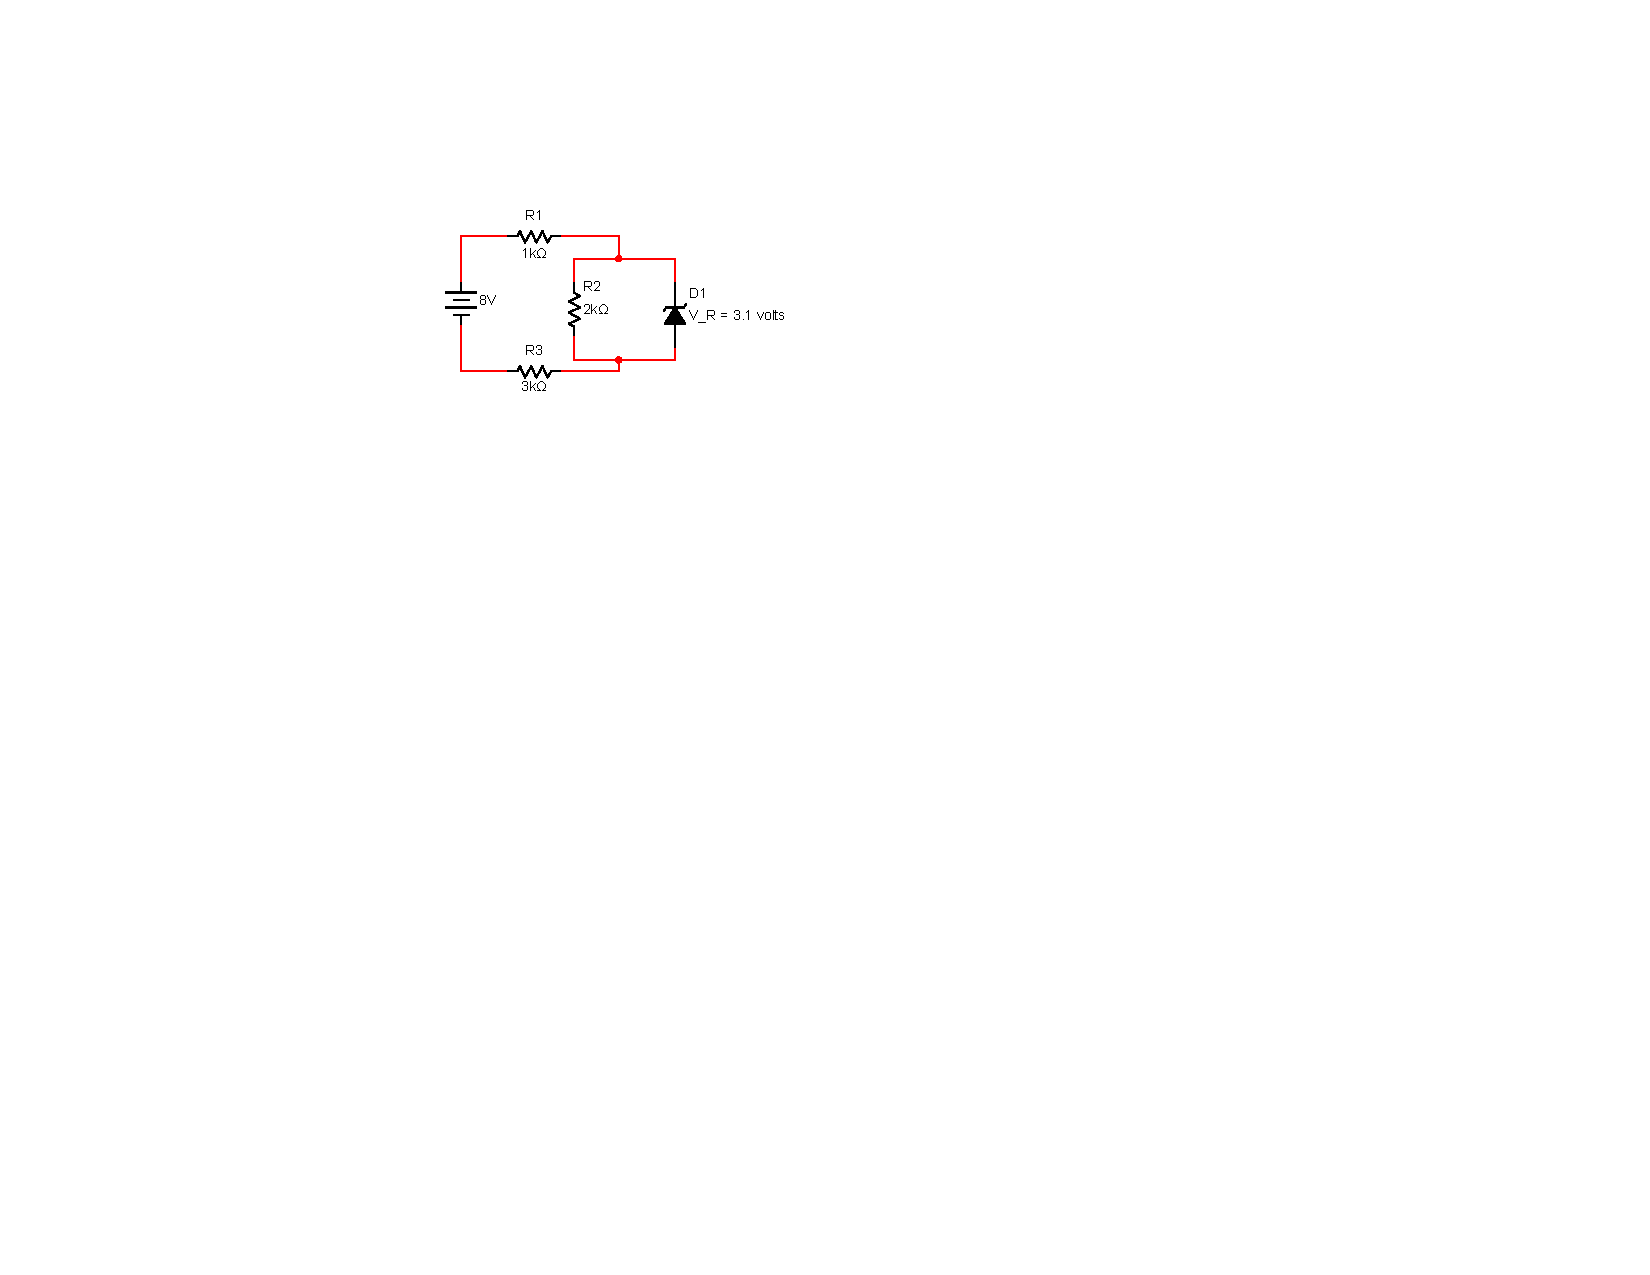
\includegraphics{M_problems/power_conversion/diode_circuit3.pdf}
\hfill\vspace*{0pt}

\hfill
\textit{Circuit diagram for \ref{prob_diode_1_of_2}}
\hfill
\textit{Circuit diagram for \ref{prob_diode_2_of_2}}
\hfill\vspace*{0pt}
\end{Exercise}
\begin{Answer}
$V_{R1}=2.2~\text{V};
V_{R2}=3.1~\text{V};
V_{R3}=6.7~\text{V};
I_{R1}=I_{R3}=2.2 ~\text{mA};
I_{R2}=1.6 ~\text{mA};
I_D=0.6 ~\text{mA}$ 
\end{Answer}


%--------------------------------------------------------------------------------------------------------------
\begin{Exercise}
\label{prob_diode_2_of_2}
In the figure above on the right, the 12~V power supoply from the previous circuit has been replaced with an 8~V power supply.  Find the voltages and currents for all resistors and for the diode.\end{Exercise}
\begin{Answer}
$V_{R1}=1.33~\text{V};
V_{R2}=2.67 ~\text{V};
V_{R3}=4.0~\text{V};
I_{R1}=I_{R2}=I_{R3}=1.33~\text{V};
I_D=0$
\end{Answer}


%--------------------------------------------------------------------------------------------------------------
\begin{Exercise}
Design two clipper circuits (series or shunt, your choice) for each of the following tasks: 
\begin{enumerate}[label=(\alph*)]
\item The first circuit should accept an input of $-10~\text{V} < V_\text{in}  < +10~\text{V}$ and produce an output that is generally positive, clipping the negative part.  For this, you don't particularly care whether the exact threshold for clipping is 0.0 or $\pm0.7$~V, but you do care that for $V_\text{in}$ above the threshold, $V_\text{in}$ and $V_\text{out}$ should differ by no more than 0.5\%.  The load for this application will be about $R_\text{load}= 50\kohm$.  
\item The second circuit should also accept an input of $-10~\text{V}<V_\text{in}< +10~\text{V}$, but should produce an output that is generally negative, clipping the positive part.  You don't care about the precision of the output much: either the exact clipping threshold or the exact ratio of  $V_\text{out}/V_\text{in}$. But this circuit will be used for $R_\text{load}= 50\ohm$, drawing up to 200~mA.  Make sure that your circuit can handle this current.
\end{enumerate}
\end{Exercise}

%--------------------------------------------------------------------------------------------------------------
\begin{Exercise}
Find the instantaneous power dissipated in the diode in the circuit below (a)~when $V_\text{in}=+5$~volts, and (b)~when $V_\text{in}=-5$~volts.

\begin{center}
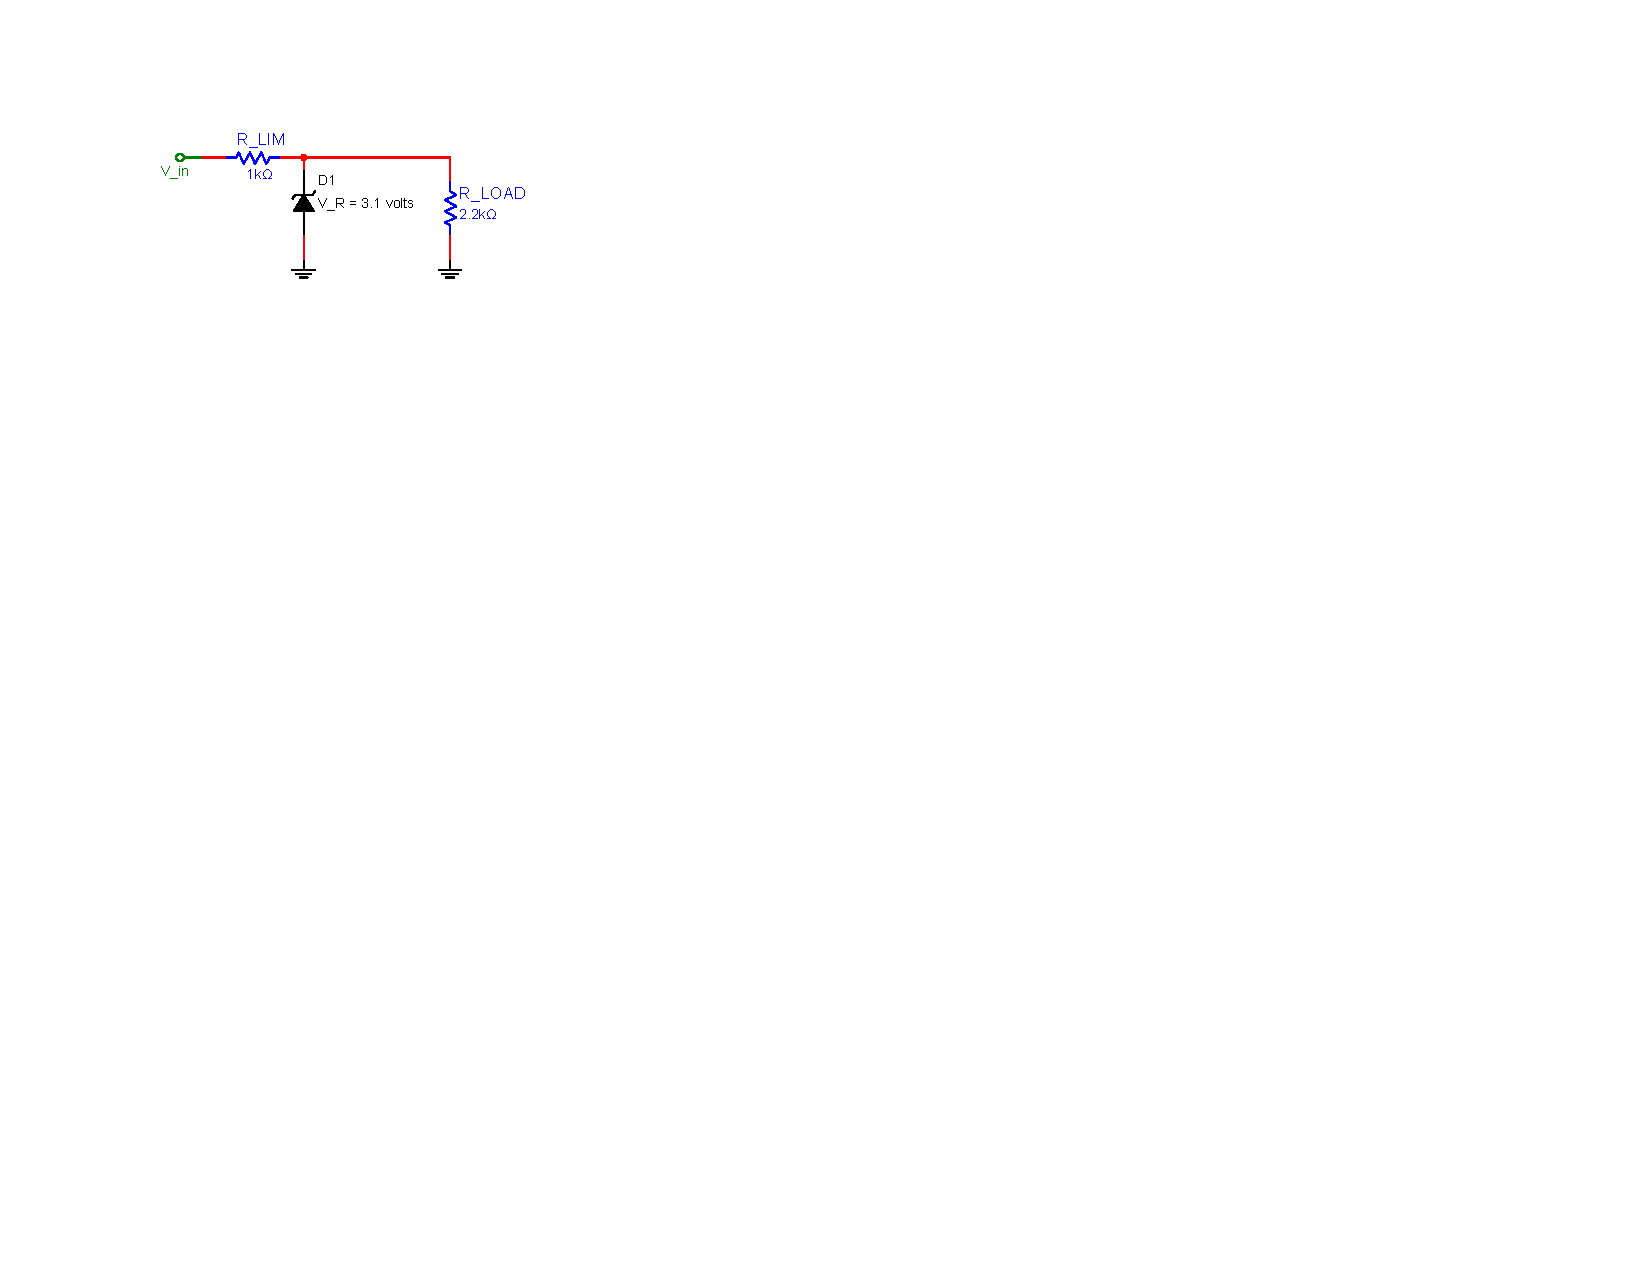
\includegraphics{M_problems/power_conversion/power_in_shunt_diode.pdf}
\end{center}
\end{Exercise}
\begin{Answer}
(a) 1.52 mW (b) 2.79 mW
\end{Answer}


%--------------------------------------------------------------------------------------------------------------
\begin{Exercise}
The diagram below shows part of a circuit inside of an actual screw-in LED light bulb.  The AC voltage input $V_\text{in}$ has already been reduced from 120 volts RMS to something smaller.  With the bulb turned on, the voltage across the capacitor is measured to have an average (DC) level of 28.7~volts and a ripple voltage of 3.4~volts.  (a)~Rewrite your expression for ripple voltage you derived in the lab in terms of the maximum current $I_\text{max}$ instead of $V_\text{max}$.  (b)~For small ripple voltages, $I_\text{max} \approx I_\text{avg}$  In fact, in your derivation, you used $\Delta Q = I \Delta t$.  Which $I$ is technically more accurate there, $I_\text{max}$ or $I_\text{avg}$? (c)~Based on the measurements given, find a numerical value for the average current through the LEDs.  (d)~Find the total power dissipated by the LEDs (some of which, presumably, is in the form of visible light).  (e)~Find the peak input voltage $V_\text{in}$ required to make the bulb work as measured above.  

\begin{center}
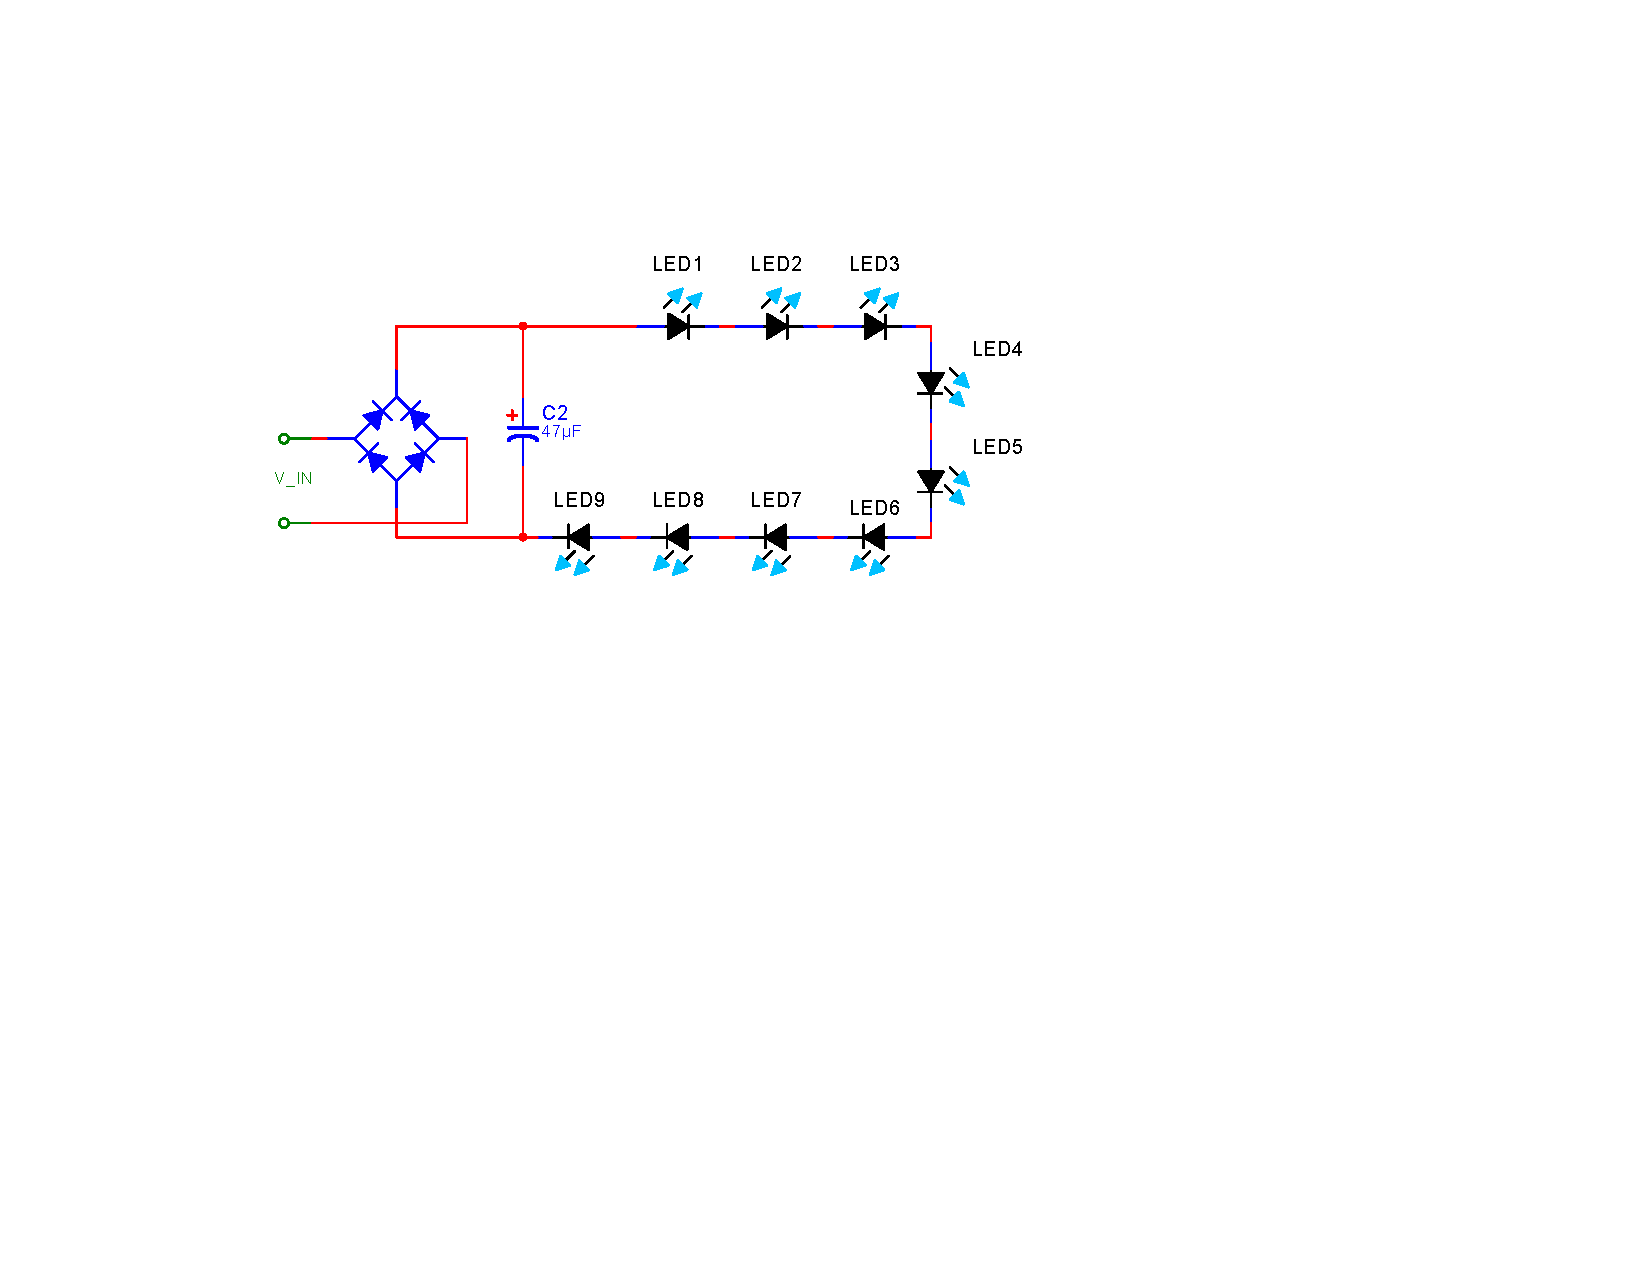
\includegraphics{M_problems/power_conversion/led_bulb_prob1.pdf}
\end{center}

\end{Exercise}
\begin{Answer}
(b) $I_\text{avg}$  (c) 19 mA (d) 0.55 watts (e) 31.8 V
\end{Answer}

%--------------------------------------------------------------------------------------------------------------
\begin{Exercise}
In the circuit below, a Zener shunt clipper is being used to regulate the voltage across $R_\text{load}=1.6\kohm$.  The input voltage $V_\text{in}$ varies sinusoidally between 7.5 and 9.0~volts.  
(a)~What value of $R_\text{lim}$ is required for the circuit to function properly, and is that a minimum or a maximum value for $R_\text{lim}$?  
(b)~Assuming the value of $R_\text{lim}$ from the last part is chosen, what is the average current through the diode?  
(c)~What is the maximum instantaneous power in both $R_\text{lim}$ and the diode?
\begin{center}
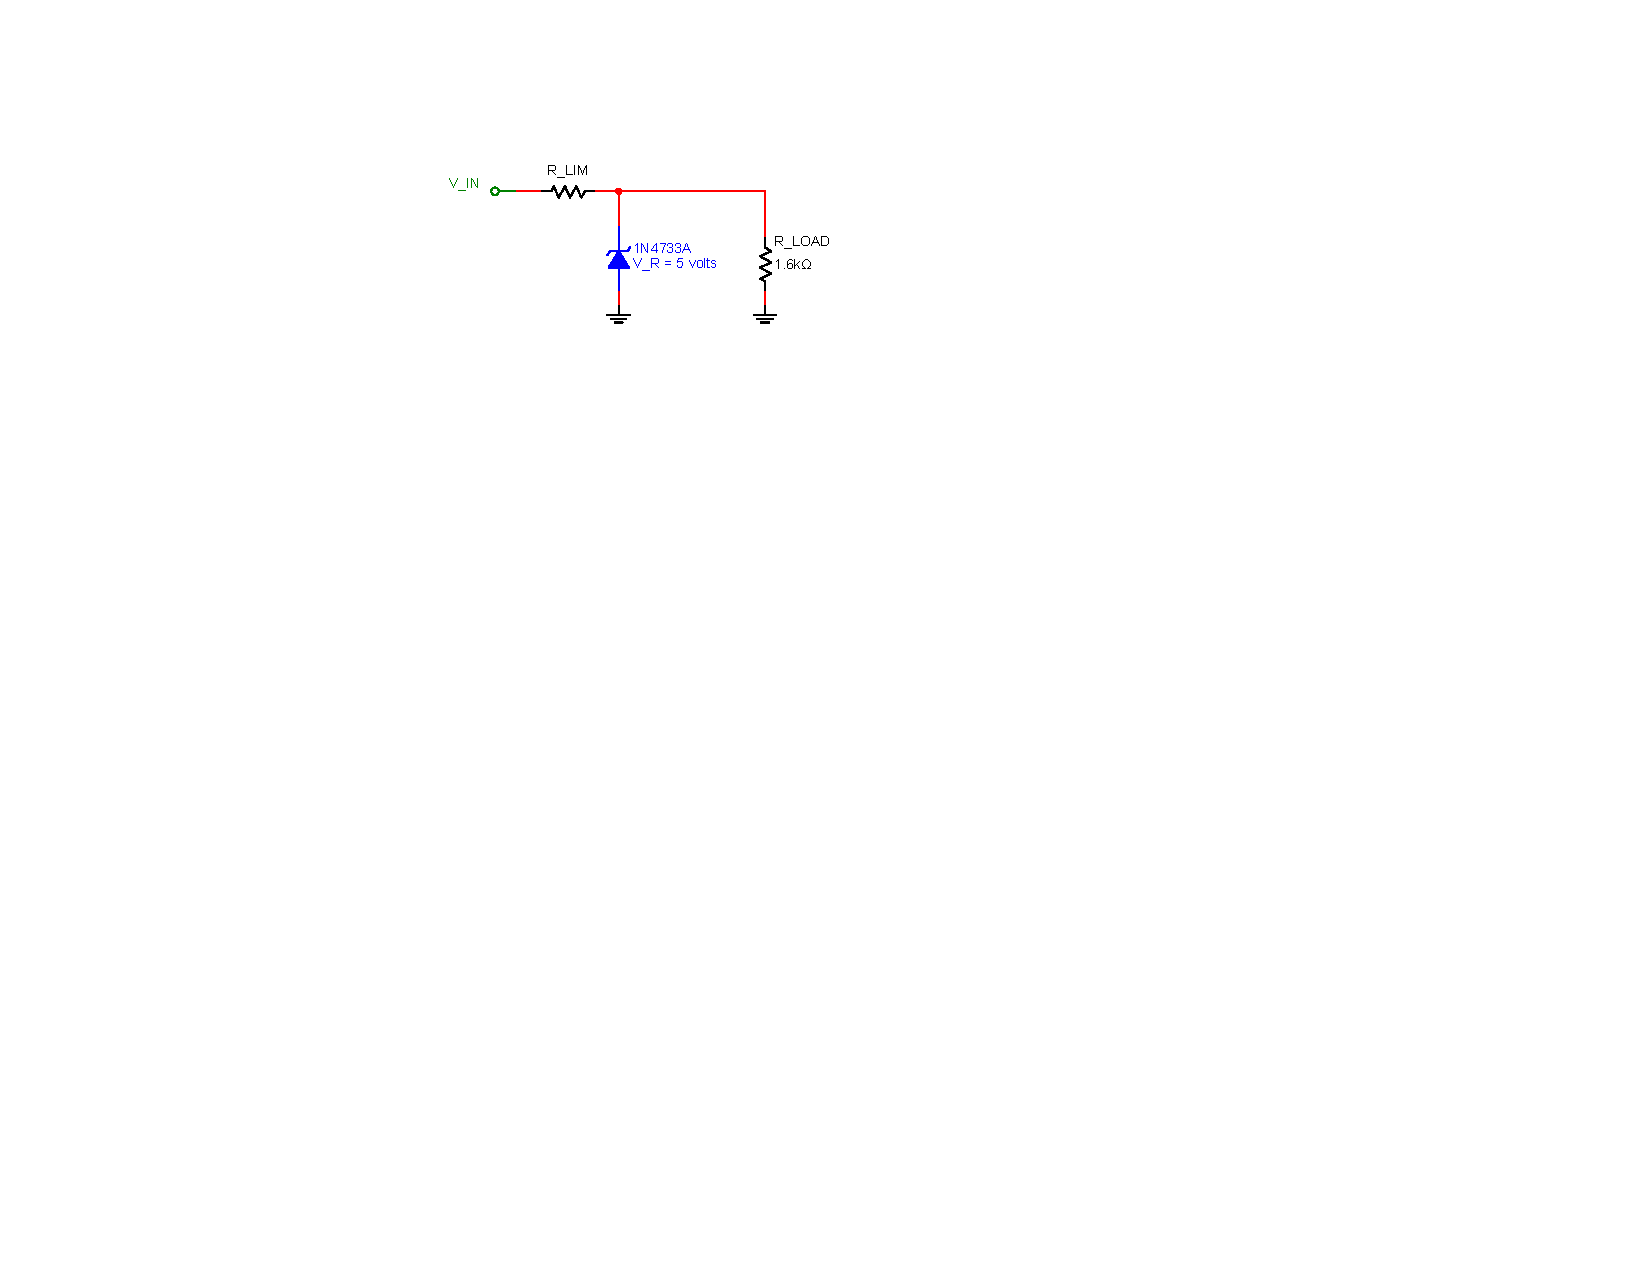
\includegraphics{M_problems/power_conversion/shunt_clipper_dc_prob.pdf}
\end{center}
\end{Exercise}
\begin{Answer}
(a) Max value of $R_\text{lim}$ is $800\ohm$. (b)~$938~\mu$A (c)~20~mW and 9.38~mW, respectively
\end{Answer}

%--------------------------------------------------------------------------------------------------------------
\begin{Exercise}
This problem will step you through process of designing a 5-volt DC power supply that can supply up to 1~amp of current, with a ripple voltage of less than 2~mV.  You will use a full wave bridge rectifier and an MC7805 regulator, which has an output voltage of 5~V, a dropout voltage of 2~V, and a minimum ripple rejection of 62~dB.  
(a)~What is the minimum instantaneous input voltage for the regulator?  
(b)~What is the minimum ripple voltage at the input of the regulator to keep the output ripple from exceeding 2~mV?  
(c)~What value of capacitor is required to maintain that ripple voltage?  
(d)~What is the peak output voltage required from the transformer?  
(e)~Assume the AC line is nominally 120~volts RMS, but might drop as low as 105~volts.  What turns-ratio transformer is required to ensure a stable 5~V output?
\end{Exercise}
\begin{Answer}
(a) 7 V (b) 2.52 V (c) $3300~\mu$F (d) 10.92 V (e) maximum of 13.6:1 
\end{Answer}



%--------------------------------------------------------------------------------------------------------------
\begin{Exercise}
The diagram below shows a clipper circuit with two Zener diodes. 
\begin{enumerate}[label=(\alph*),nosep]
\item Draw a graph of the output voltage vs. time, labeling the minimum and maximum values. 
\item Calculate the maximum magnitude of the instantaneous current through the diodes. 
\item Find the maximum instantaneous power dissipated in diode $D_2$ and in the resistor $R_\text{lim}$.
\end{enumerate}
\begin{center}
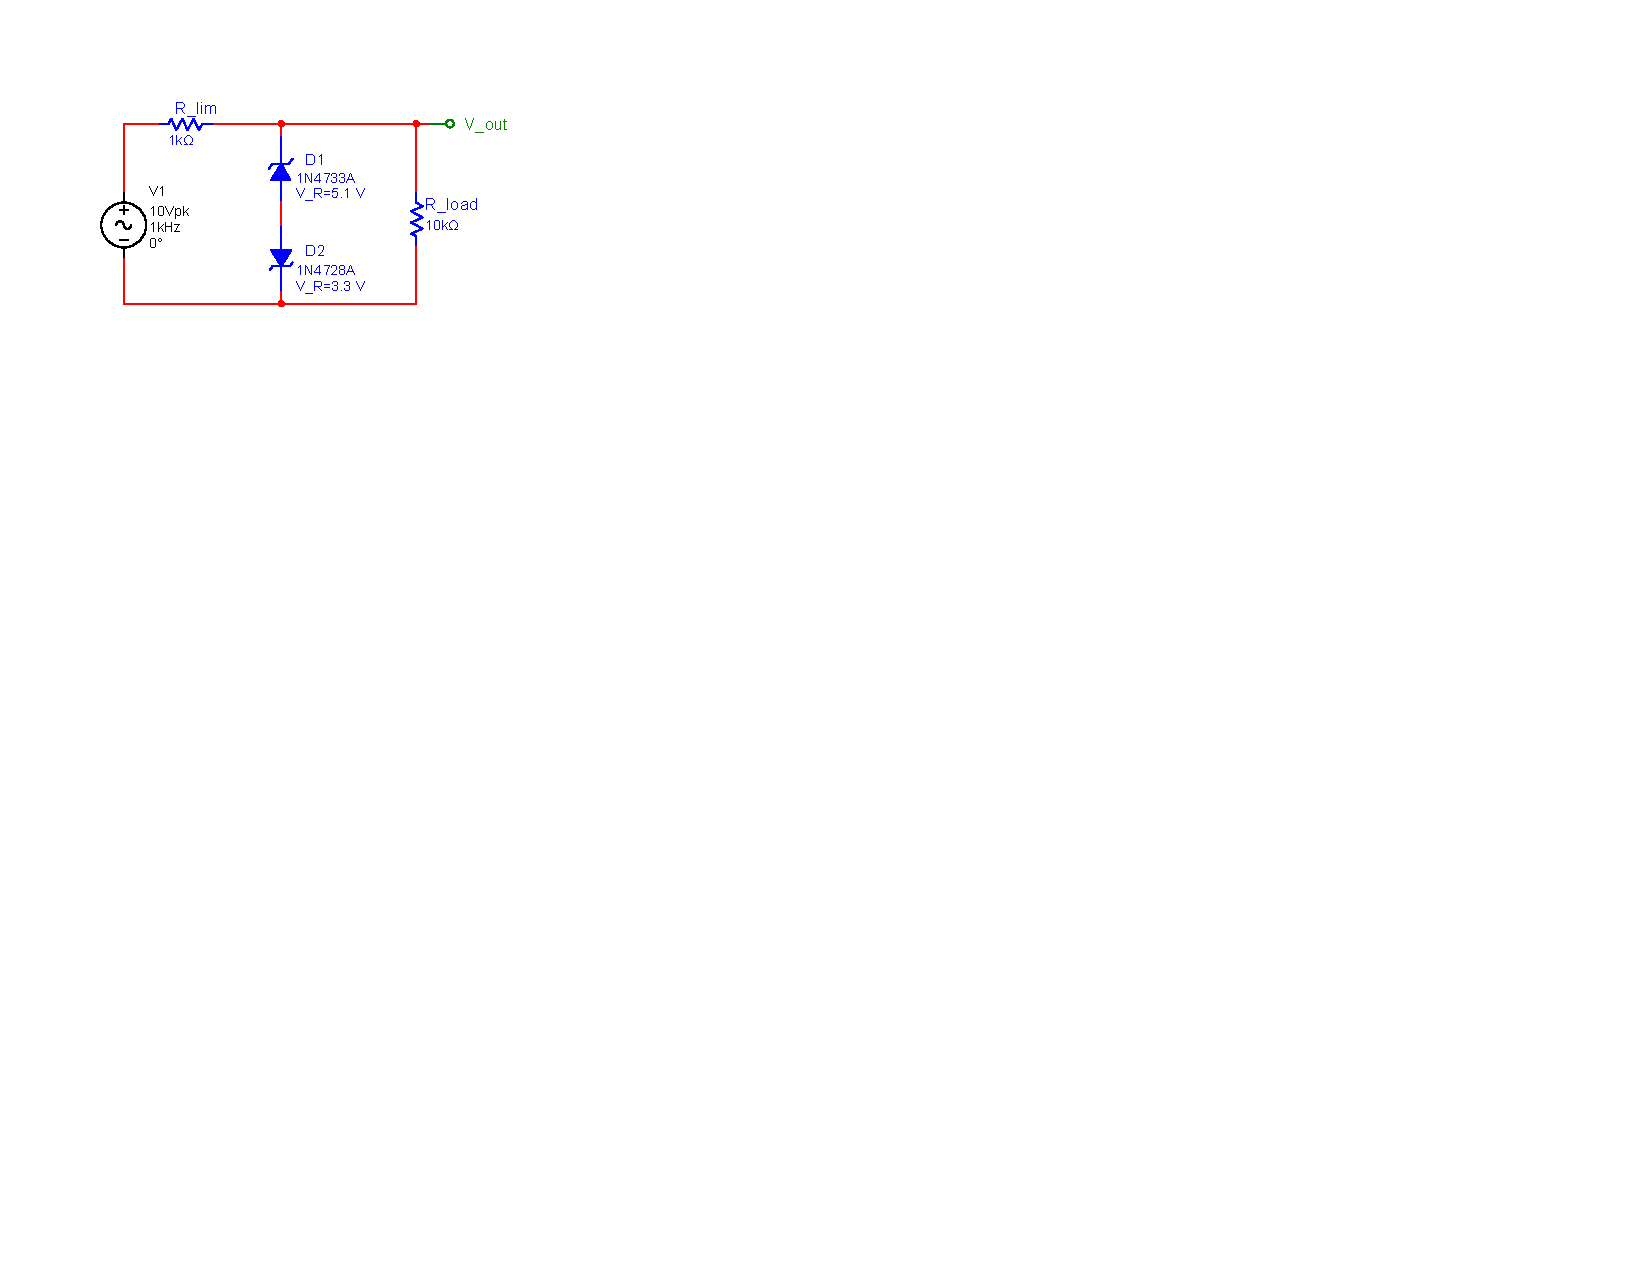
\includegraphics{M_problems/power_conversion/double_zener_shunt_clipper_prob.pdf}
\end{center}
\end{Exercise}
\begin{Answer}
(b) 5.6 mA (c) 18.5 mW and 36 mW.
\end{Answer}


%Ideas for additional problems:
%\vfill
%\pagebreak[3]

\vspace{0.7in}

\textbf{Answers to Selected {\thesubsection} Problems:}
\label{power_conversion_prob_answers}
%\shipoutExercise
\shipoutAnswer

\cleardoublepage
